\documentclass[cn,hazy,blue,pad,14pt]{elegantnote}
\newtheorem{ti}{}
\renewcommand{\theti}{\arabic{ti}.}
\usepackage{tikz}
\usetikzlibrary{ducks}
\usepackage[siunitx,RPvoltages]{circuitikz}
\title{《电工电子技术》2019-2020 考试卷\thanks{试卷编号:1920010622A,秋,32 课时.江理学习资料库:\href{https://github.com/sikouhjw/jxust-Learning-database}{GitHub} or \href{https://gitee.com/sikouhjw/jxust-Learning-database}{Gitee}.}}
\author{秦淑雅}
% \institute{\url{https://github.com/sikouhjw/jxust-Learning-database} \\ \url{https://gitee.com/sikouhjw/jxust-Learning-database}}
% \version{1.00}
\date{\zhtoday}
\def\jj{\mathrm{j}}
\def\LL{\mathrm{L}}
\def\ii{\mathrm{i}}
\def\oo{\mathrm{o}}
\begin{document}
\maketitle
\section{致谢}
感谢 \href{https://github.com/ElegantLaTeX/ElegantNote}{ElegantNote} 提供的模板,Happy LaTeXing!~
\section{正文}
\begin{ti}[12 分]
	求电压 $u$,并求 \SI{3}{V} 电压源和 \SI{1}{A} 电流源功率及判断其性质.
	\begin{center}
		\begin{circuitikz}[european]
			\ctikzset{voltage=american}
			\draw (0,0) to[V,V=\SI{3}{V}] ++ (0,2) -- ++ (2,0) to[R,R=\SI{2}{\Omega},v=$u$] ++ (0,-2) -- ++ (-2,0);
			\draw (2,0) -- ++ (2,0) to[I,i=\SI{1}{A}] ++ (0,2) -- ++ (-2,0);
		\end{circuitikz}
	\end{center}
\end{ti}

\begin{ti}[12 分]
	用戴维宁定理计算电流 $I$.
	\begin{center}
		\begin{circuitikz}[european]
			\draw (0,0) to[I,i=\SI{6}{A}] ++ (0,4) -- ++ (2,0) to[R,R=\SI{12}{\Omega}] ++ (0,-4) -- ++ (-2,0);
			\draw (2,4) to[R,R=\SI{2}{\Omega},i=$I$] ++ (4,0) to[R,R=\SI{6}{\Omega}] ++ (0,-4) -- ++ (-4,0);
			\draw (6,4) -- ++ (2,0) to[R,R=\SI{3}{\Omega}] ++ (0,-2) to[V,V<=\SI{12}{V}] ++ (0,-2) -- ++ (-2,0);
		\end{circuitikz}
	\end{center}
\end{ti}
\edef\aSI{$R_{1} = \SI{4}{\Omega}$}
\edef\bSI{$R_{2} = \SI{2}{\Omega}$}
\begin{ti}
	在开关闭合前电路已处于稳态,求开关闭合后的 $u_{C}$.
	\begin{center}
		\begin{circuitikz}[european]
			\draw (0,0) to[I,i=\SI{1.5}{A}] ++ (0,2) -- ++ (2,0) to[R,R=\aSI] ++ (0,-2) -- ++ (-2,0);
			\draw (2,2) -- ++ (3,0) to[C,l=$u_{C}$,name=myC] ++ (0,-2) -- ++ (-3,0);
			\node[right=10pt,below=5pt] at (myC) {$-$};
			\node[right=10pt,above=5pt] at (myC) {$+$};
			\node[right=25pt,below=10pt] at (myC) {\SI{300}{\upmu F}};
			\draw (5,0) -- ++ (2,0) to[R,l_=\bSI] ++ (0,2) to[cspst] ++ (-2,0);
		\end{circuitikz}
	\end{center}
\end{ti}

\begin{ti}
	已知电压 $U = \SI{12}{V}$,$z = (1.7 + \jj)\ \si{\Omega}$,$z_{1} = (3 + \jj 4)\ \si{\Omega}$,$z_{2} = (4 - \jj 4)\ \si{\Omega}$,求各支路电流及电路的有功功率.
	\begin{center}
		\begin{circuitikz}[european]
			\draw (0,2) to[R,R=$z$,i=$\dot{I}$] ++ (2,0) to[R,R=$z_{1}$,i=$\dot{I}_{1}$] ++ (0,-2) -- ++ (-2,0);
			\draw (2,2) -- ++ (2,0) to[R,R=$z_{2}$,i=$\dot{I}_{2}$] ++ (0,-2) -- ++ (-2,0);
			\node[left] at (0,2) {$+$};
			\node[left] at (0,0) {$-$};
			\node[left] at (0,1) {$\dot{U}$};
		\end{circuitikz}
	\end{center}
\end{ti}

\begin{ti}
	对称三相绕组为三角形联结,其线电压 $U_{\LL} = \SI{380}{V}$,线电流 $I_{\LL} = \SI{84.2}{A}$,三相负载总功率 $P = \SI{48.75}{kW}$,计算每相负载的等效复阻抗 $z$.
\end{ti}

\begin{ti}
	$u_{\ii} = 10 \sin \omega t$,二极管正向压降及反向电流均忽略不计,画出电压 $u_{\oo}$ 的波形.
	\begin{center}
		\begin{circuitikz}[european]
			\draw (0,4) to[D] ++ (2,0) to[R,R=\SI{10}{k\Omega}] ++ (0,-2) to[V,V<=\SI{5}{V}] ++ (0,-2) -- ++ (-2,0);
			\draw (2,4) -- ++ (2,0) node[right] {$+$};
			\draw (2,0) -- ++ (2,0) node[right] {$-$};
			\node[right] at (4,2) {$u_{\oo}$};
			\node[left] at (0,4) {$+$};
			\node[left] at (0,0) {$-$};
			\node[left] at (0,2) {$u_{\ii}$};
		\end{circuitikz}
	\end{center}
\end{ti}

\begin{ti}
	$\beta = 60$,$U_{\mathrm{BE}} = \SI{0.6}{V}$,$R_{\LL} = \SI{2.2}{k\Omega}$,要使静态时 $U_{\mathrm{CE}} = \SI{6}{V}$,$R_{\mathrm{B}}$ 为何值?要使 $I_{\LL} = \SI{1.5}{mA}$,$R_{\mathrm{B}}$ 为何值?
	\begin{center}
		\begin{circuitikz}[european]
			\draw (4,2) node[npn](Q){};
			\draw (0,2) to[C,C=$C_{1}$] node[xshift=-0.6cm,yshift=10pt] {$+$} ++ (2,0) -- (Q.B);
			\draw (Q.C) to[R,R=$R_{\mathrm{C}}$] ++ (0,2) -- ++ (1,0) node[right] {$V_{\mathrm{CC}} = \SI{12}{V}$} ++ (-1,0) -- ++(-1.5,0) to[tgeneric,l_=$R_{\mathrm{B}}$] (2.5,2);
			\draw (Q.C) ++ (0,0.1) to[C,C=$C_{2}$] node[xshift=-1.4cm,yshift=10pt] {$+$} ++ (2,0) to[R,l_=$R_{\LL}$] (6,0) -- (0,0);
			\draw (Q.E) -- (4,-0.5) ++ (0.25,0) -- ++ (-0.5,0);
			\node[left] at (0,0) {$-$};
			\node[left] at (0,2) {$+$};
			\node[left] at (0,1) {$\dot U_{\ii}$};
			\node[xshift=20pt] at (6,0) {$-$};
			\node[xshift=20pt] at (6,2.85) {$+$};
			\node[xshift=20pt] at (6,1.425) {$\dot U_{\oo}$};
		\end{circuitikz}
	\end{center}
\end{ti}

\begin{ti}
	分析下图所示电路的逻辑功能.
	\begin{center}
		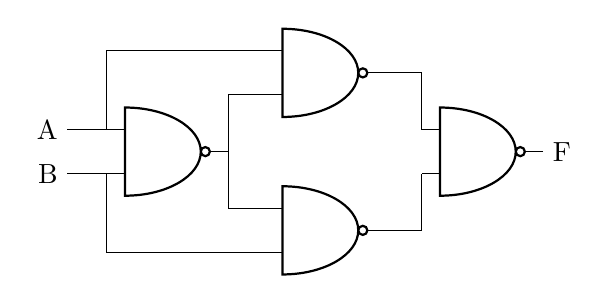
\begin{tikzpicture}[american ports]
			\draw (2,0) node[nand port] (A) {};
			\draw (4,1) node[nand port] (B) {};
			\draw (4,-1) node[nand port] (C) {};
			\draw (6,0) node[nand port] (D) {};
			\draw (A.in 1) -- ++ (-0.5,0) node[left] {A};
			\draw (A.in 2) -- ++ (-0.5,0) node[left] {B};
			\draw (A.out) |- (B.in 2);
			\draw (A.out) |- (C.in 1);
			\draw (B.out) -| (D.in 1);
			\draw (C.out) -| (D.in 2);
			\draw (A.in 1) |- (B.in 1);
			\draw (A.in 2) |- (C.in 2);
			\node[right] at (D.out) {F};
		\end{tikzpicture}
	\end{center}
\end{ti}

\begin{ti}
	基本 RS 触发器如下图,根据图~b 的输入波形画出 $Q$ 的波形.设触发器初始状态 $Q = 0$.
	\begin{center}
		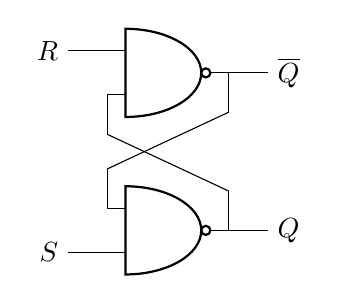
\begin{tikzpicture}[american ports]
			\draw (0,2) node[nand port] (A) {};
			\draw (0,0) node[nand port] (B) {};
			\draw (A.in 1) -- ++ (-0.5,0) node[left] {$R$};
			\draw (B.in 2) -- ++ (-0.5,0) node[left] {$S$};
			% \node[left] at (A.in 1) {$R$};
			% \node[left] at (B.in 2) {$S$};
			\draw (A.in 2) -- ++ (0,-0.5) coordinate (a);
			\draw (B.in 1) -- ++ (0,0.5) coordinate (b);
			\draw (A.out) -- ++ (0,-0.5) coordinate (c);
			\draw (B.out) -- ++ (0,0.5) coordinate (d);
			\draw (a) -- (d);
			\draw (b) -- (c);
			\draw (A.out) -- ++ (0.5,0) node[right] {$\overline{Q}$};
			\draw (B.out) -- ++ (0.5,0) node[right] {$Q$};
		\end{tikzpicture}
		\begin{tikzpicture}
			\draw (0,0) node[left] {$S$} -- ++ (1,0) -- ++ (0,1) -- ++ (2,0) -- ++ (0,-1) -- ++ (1,0) -- ++ (0,1) -- ++ (1,0) -- ++ (0,-1) -- ++ (1,0);
			\draw (0,-1) node[left] {$R$} -- ++ (1,0) -- ++ (0,-1) -- ++ (1,0) |- ++ (0.5,1) |- ++ (0.5,-1) |- ++ (1,1) |- ++ (2,-1);
		\end{tikzpicture}
	\end{center}
\end{ti}
\end{document}